% SDRTerm — ADS-B (1090 MHz Mode S) pipeline walkthrough
%
% Build with:  pdflatex pipeline.tex   (twice, so ToC + refs resolve)

\documentclass[11pt,a4paper]{article}

\usepackage[margin=2cm]{geometry}
\usepackage{amsmath,amssymb,amsthm}
\usepackage{tikz}
\usepackage{pgfplots}
\pgfplotsset{compat=1.18}
\usetikzlibrary{arrows.meta, positioning, shapes.geometric, calc,
                decorations.pathreplacing, backgrounds, fit, patterns}
\usepackage{listings}
\usepackage{xcolor}
\usepackage{hyperref}
\usepackage{caption}
\usepackage{booktabs}
\usepackage{siunitx}
\usepackage{parskip}

\hypersetup{
  colorlinks=true,
  linkcolor=blue!70!black,
  urlcolor=blue!60!black,
  citecolor=black,
}

\lstset{
  basicstyle=\ttfamily\small,
  frame=single,
  breaklines=true,
  showstringspaces=false,
  columns=fullflexible,
  keepspaces=true,
  backgroundcolor=\color{gray!5},
}

\title{ADS-B Signal Capture and Processing\\
       \large A Mathematical Walkthrough of SDRTerm's \texttt{adsb} Plugin}
\author{SDRTerm project}
\date{\today}

\begin{document}
\maketitle
\tableofcontents
\vspace{2em}

%═══════════════════════════════════════════════════════════════════
\section{Introduction}
%═══════════════════════════════════════════════════════════════════

\emph{Automatic Dependent Surveillance -- Broadcast} (ADS-B) is the
open-format position-broadcasting system every commercial aircraft in
controlled airspace is required to run.  Each aircraft transmits its own
identity, position, altitude and velocity twice a second on the
\SI{1090}{MHz} Mode~S reply channel.  Because the signal is
unencrypted and short, a small antenna, an LNA, and any SDR that can
tune \SI{1090}{MHz} at \SI{2}{MSPS} or better is enough to decode traffic
overhead for tens of kilometres.

The chain, from antenna to on-screen aircraft table, has five stages:

\begin{center}
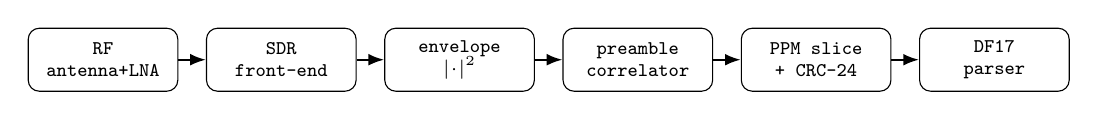
\begin{tikzpicture}[node distance=0.35cm,
  block/.style={draw, rounded corners, minimum width=1.9cm, minimum height=0.8cm,
                align=center, font=\scriptsize\ttfamily},
  arrow/.style={-{Latex[length=2mm]}, thick}]

  \node[block] (rf)      {RF\\antenna+LNA};
  \node[block, right=of rf]      (sdr)  {SDR\\front-end};
  \node[block, right=of sdr]     (env)  {envelope\\$|\!\cdot\!|^2$};
  \node[block, right=of env]     (pre)  {preamble\\correlator};
  \node[block, right=of pre]     (dem)  {PPM slice\\+ CRC-24};
  \node[block, right=of dem]     (par)  {DF17\\parser};

  \draw[arrow] (rf)  -- (sdr);
  \draw[arrow] (sdr) -- (env);
  \draw[arrow] (env) -- (pre);
  \draw[arrow] (pre) -- (dem);
  \draw[arrow] (dem) -- (par);
\end{tikzpicture}
\end{center}

Design differences vs.\ Iridium (see the sibling \texttt{iridium\_decoder}
walkthrough):

\begin{itemize}
  \item \textbf{Modulation is simple.} On/off keying at \SI{1}{Mbit/s} --
        pulse in the first half of a symbol slot means bit~1, in the
        second half means bit~0.  No carrier phase to track, no PLL.
  \item \textbf{No FEC.} Only a \SI{24}{bit} CRC that
        \emph{doubles} as an address field for downlink formats where the
        ICAO24 has been XOR'd into the parity.
  \item \textbf{Traffic is dense.} Over a busy airport you may see hundreds
        of squitters per second -- decoding must be cheap per burst.
  \item \textbf{Position is compact.} CPR (Compact Position Reporting)
        squeezes lat/lon into $17 + 17$ bits at the cost of an
        even/odd-frame pairing rule the receiver must implement.
\end{itemize}

%═══════════════════════════════════════════════════════════════════
\section{Signal Basics}
%═══════════════════════════════════════════════════════════════════

\subsection{Complex baseband on 1090\,MHz}

The transponder emits a real-valued RF burst
$s_{\text{RF}}(t) = A(t)\cos(2\pi f_c t + \phi)$
with $f_c = \SI{1090}{MHz}$.  The SDR mixes down to complex baseband
\begin{equation}
x(t) = I(t) + j Q(t)\quad\in\quad\mathbb{C},
\end{equation}
so that the pulse envelope $|x(t)|$ approximates the transmitted
amplitude $A(t)$.  Because ADS-B is amplitude-only, we discard phase
information straight away:
\begin{equation}
e[n] = |x[n]|^{2} = I[n]^{2} + Q[n]^{2}.
\end{equation}
Using $|x|^2$ instead of $|x|$ saves a square-root per sample and turns
the correlator that follows into a linear operation on power.

\begin{center}
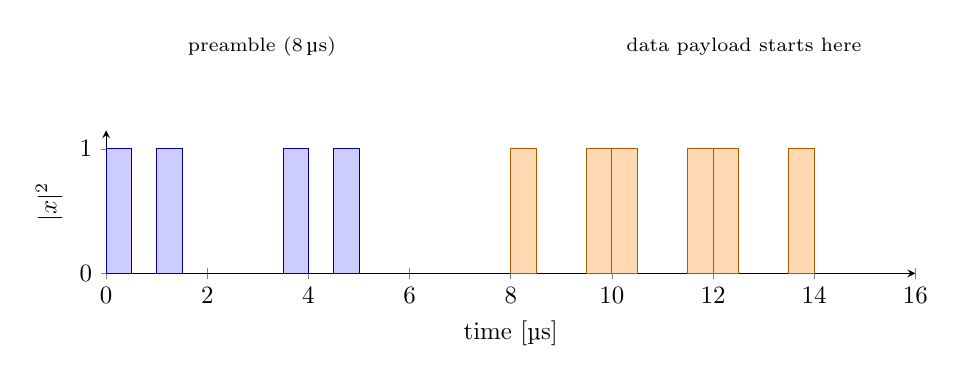
\begin{tikzpicture}[scale=0.90]
  \begin{axis}[width=13cm, height=3.6cm, ymin=0, ymax=1.15,
    xlabel={time [\si{\micro\second}]}, ylabel={$|x|^{2}$},
    axis y line=left, axis x line=bottom,
    xmin=0, xmax=16, xtick={0,2,4,6,8,10,12,14,16},
    ytick={0,1}]
    % Preamble pulses at 0, 1, 3.5, 4.5 (each 0.5 µs wide)
    \addplot[fill=blue!20, draw=blue!60!black] coordinates {(0,0)(0,1)(0.5,1)(0.5,0)} \closedcycle;
    \addplot[fill=blue!20, draw=blue!60!black] coordinates {(1,0)(1,1)(1.5,1)(1.5,0)} \closedcycle;
    \addplot[fill=blue!20, draw=blue!60!black] coordinates {(3.5,0)(3.5,1)(4,1)(4,0)} \closedcycle;
    \addplot[fill=blue!20, draw=blue!60!black] coordinates {(4.5,0)(4.5,1)(5,1)(5,0)} \closedcycle;
    % Data bits (illustrative pattern 1010 0110)
    \addplot[fill=orange!30, draw=orange!70!black] coordinates {(8,0)(8,1)(8.5,1)(8.5,0)} \closedcycle;
    \addplot[fill=orange!30, draw=orange!70!black] coordinates {(9.5,0)(9.5,1)(10,1)(10,0)} \closedcycle;
    \addplot[fill=orange!30, draw=orange!70!black] coordinates {(10,0)(10,1)(10.5,1)(10.5,0)} \closedcycle;
    \addplot[fill=orange!30, draw=orange!70!black] coordinates {(11.5,0)(11.5,1)(12,1)(12,0)} \closedcycle;
    \addplot[fill=orange!30, draw=orange!70!black] coordinates {(12,0)(12,1)(12.5,1)(12.5,0)} \closedcycle;
    \addplot[fill=orange!30, draw=orange!70!black] coordinates {(13.5,0)(13.5,1)(14,1)(14,0)} \closedcycle;
  \end{axis}
  \node[font=\scriptsize] at (2.2,3.2) {preamble (\SI{8}{\micro\second})};
  \node[font=\scriptsize] at (9.0,3.2) {data payload starts here};
\end{tikzpicture}
\end{center}

\subsection{Sample rate and Nyquist}

The information bandwidth of ADS-B is $\sim\SI{4}{MHz}$ (the pulses
have $\sim\SI{0.5}{\micro\second}$ rise and fall times), but for
detection we only need enough samples per bit to distinguish the first-half
from the second-half of each \SI{1}{\micro\second} symbol.  The minimum
useful rate is therefore
\begin{equation}
f_s^{\min} = 2 \cdot B_{\text{bit}} = \SI{2}{MSPS},
\end{equation}
giving 2 samples per bit.  Higher rates -- \SI{2.4}{MSPS} for an
RTL-SDR (\texttt{dump1090-style}) or \SI{8}{MSPS} for an
Airspy -- give more preamble timing resolution and better decode rate
under weak signals or overlapping frames.

\begin{center}
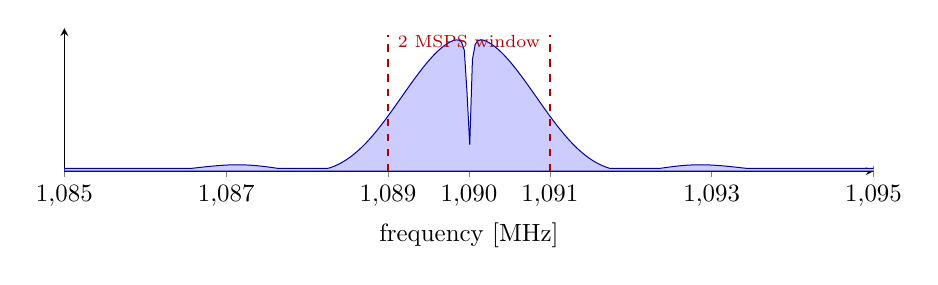
\begin{tikzpicture}[scale=0.90]
  \begin{axis}[width=13cm, height=3.6cm, ymin=0, ymax=1.05,
    xlabel={frequency [\si{MHz}]}, ylabel={},
    xmin=1085, xmax=1095, xtick={1085,1087,1089,1090,1091,1093,1095},
    ytick={\empty}, axis y line=left, axis x line=bottom]
    % Spectral density of ADS-B (approx sinc^2 around 1090)
    \addplot[domain=1085:1095, samples=300, fill=blue!20, draw=blue!60!black]
      {max(0.02, (sin(deg(pi*(x-1090)/2))^2)/((pi*(x-1090)/2)^2 + 0.001))} \closedcycle;
    % Tuner acceptance window ±1 MHz (2 MSPS)
    \draw[dashed, red!70!black, thick]
      (axis cs:1089,0) -- (axis cs:1089,1);
    \draw[dashed, red!70!black, thick]
      (axis cs:1091,0) -- (axis cs:1091,1);
    \node[font=\scriptsize, red!70!black] at (axis cs:1090,0.95) {2 MSPS window};
  \end{axis}
\end{tikzpicture}
\end{center}

The dashed lines show a \SI{2}{MSPS} window centred on \SI{1090}{MHz}:
$\pm\SI{1}{MHz}$ of usable bandwidth -- narrow enough to reject the
neighbouring GPS and DME channels, wide enough to keep the ADS-B pulse
main lobe.

%═══════════════════════════════════════════════════════════════════
\section{Physical layer of Mode~S}
%═══════════════════════════════════════════════════════════════════

\subsection{Frame layout}

Every downlink squitter has three parts:

\begin{center}
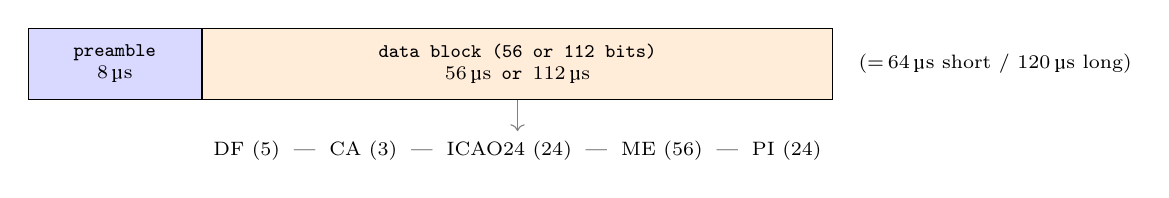
\begin{tikzpicture}[node distance=0mm,
  block/.style={draw, minimum height=0.9cm, align=center, font=\scriptsize\ttfamily},
]
  \node[block, fill=blue!15, minimum width=2.2cm]                    (p)  {preamble\\\SI{8}{\micro s}};
  \node[block, fill=orange!15, minimum width=8.0cm, right=0mm of p]  (d)  {data block (56 or 112 bits)\\\SI{56}{\micro s} or \SI{112}{\micro s}};
  \node[right=0.2cm of d, font=\scriptsize] {(=\,\SI{64}{\micro s} short / \SI{120}{\micro s} long)};

  % Fields within long msg
  \node[below=0.4cm of d, font=\scriptsize] (label) {DF (5) \;|\; CA (3) \;|\; ICAO24 (24) \;|\; ME (56) \;|\; PI (24)};
  \draw[->, gray] (d.south) -- (label.north);
\end{tikzpicture}
\end{center}

\begin{itemize}
  \item \textbf{DF} -- \emph{downlink format}, 5 bits.  \texttt{17} is ADS-B
        extended squitter (the one we want); \texttt{11} is a short reply,
        \texttt{4} / \texttt{5} / \texttt{20} / \texttt{21} are Mode-A/C
        replies still occasionally seen.
  \item \textbf{CA} -- capability field, 3 bits.
  \item \textbf{ICAO24} -- the aircraft's globally unique
        \SI{24}{bit} hex identifier (e.g.\ \texttt{4CA1F2}).
  \item \textbf{ME} -- 56-bit \emph{message extension} whose content
        depends on the top 5 bits (the \emph{type code}, TC).
  \item \textbf{PI} -- 24-bit parity/interrogator field.  For DF17 it is
        the CRC-24 of the preceding 88 bits, unmodified; for DF11 it is
        the CRC XOR'd with the interrogator address.
\end{itemize}

\subsection{Preamble structure}

The preamble is a fixed sequence of four \SI{0.5}{\micro s} pulses at
\SI{0.0}{\micro s}, \SI{1.0}{\micro s}, \SI{3.5}{\micro s} and
\SI{4.5}{\micro s} from the frame start:

\begin{center}
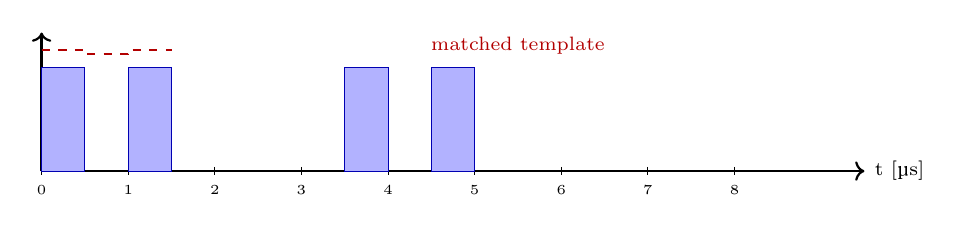
\begin{tikzpicture}[scale=1.1]
  \draw[->, thick] (0,0) -- (9.5,0) node[right, font=\scriptsize]{t [\si{\micro\second}]};
  \draw[->, thick] (0,0) -- (0,1.6);
  \foreach \x/\lbl in {0/0, 1/1, 2/2, 3/3, 4/4, 5/5, 6/6, 7/7, 8/8}{
    \draw (\x,0.05)--(\x,-0.05) node[below, font=\tiny]{\lbl};
  }
  % four pulses
  \foreach \a/\b in {0/0.5, 1/1.5, 3.5/4.0, 4.5/5.0}{
    \filldraw[fill=blue!30, draw=blue!70!black] (\a,0) rectangle (\b,1.2);
  }
  % Correlator template overlay
  \draw[red!70!black, dashed, thick]
    (0,1.4) -- (0.5,1.4) -- (0.5,1.35) -- (1,1.35) -- (1,1.4) -- (1.5,1.4);
  \node[red!70!black, font=\scriptsize] at (5.5,1.45) {matched template};
\end{tikzpicture}
\end{center}

Any energy in the ``dead'' slots at $[0.5,1.0]$, $[1.5,3.5]$,
$[4.0,4.5]$ or $[5.0,8.0]$~$\si{\micro s}$ makes a candidate less
preamble-like -- the correlator (\S\ref{sec:preamble}) exploits this.

\subsection{Pulse-position modulation of data}

Each data bit occupies a \SI{1}{\micro s} slot.  A pulse in the first
half ($[0, 0.5]$~$\si{\micro s}$) codes bit~1, in the second half
($[0.5, 1.0]$~$\si{\micro s}$) codes bit~0:

\begin{center}
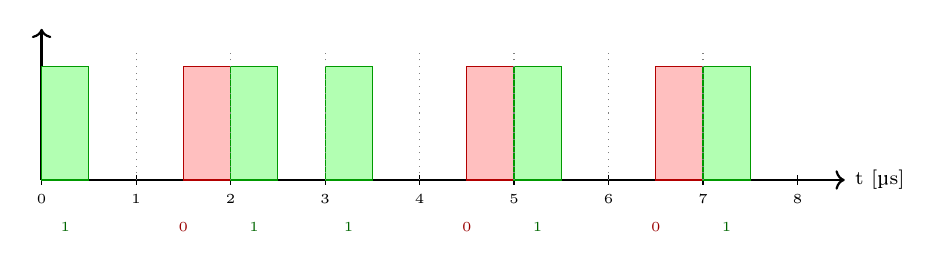
\begin{tikzpicture}[scale=1.2]
  \draw[->, thick] (0,0) -- (8.5,0) node[right, font=\scriptsize]{t [\si{\micro\second}]};
  \draw[->, thick] (0,0) -- (0,1.6);
  \foreach \x in {0,...,8}{
    \draw (\x,0.05)--(\x,-0.05) node[below, font=\tiny]{\x};
  }
  % Bits 1 0 1 1 0 1 0 1 → pulses at first/second halves
  \foreach \x/\bit in {0/1, 1/0, 2/1, 3/1, 4/0, 5/1, 6/0, 7/1}{
    \ifnum\bit=1
      \filldraw[fill=green!30, draw=green!60!black] (\x,0) rectangle (\x+0.5,1.2);
      \node[font=\tiny, green!40!black] at (\x+0.25,-0.5) {1};
    \else
      \filldraw[fill=red!25, draw=red!70!black] (\x+0.5,0) rectangle (\x+1,1.2);
      \node[font=\tiny, red!60!black] at (\x+0.5,-0.5) {0};
    \fi
  }
  % slot boundaries
  \foreach \x in {1,...,7}{
    \draw[gray, dotted] (\x,0)--(\x,1.4);
  }
\end{tikzpicture}
\end{center}

For a receiver this is beautifully simple.  Sum the sample power in the
first half-slot ($P_0$) and in the second half-slot ($P_1$):
\begin{equation}
b_k = \begin{cases} 1 & P_0 > P_1 \\ 0 & \text{otherwise} \end{cases}
\qquad
P_0 = \!\!\!\!\!\sum_{n=k\cdot sps}^{k\cdot sps+sps/2 - 1}\!\!\!\!e[n],
\quad
P_1 = \!\!\!\!\!\!\!\sum_{n=k\cdot sps+sps/2}^{(k+1)\cdot sps - 1}\!\!\!\!e[n],
\end{equation}
where $sps$ is samples per symbol ($= f_s / \SI{1}{Mbit/s}$ = 2 at
\SI{2}{MSPS}, 8 at \SI{8}{MSPS}).  No PLL, no matched filter, no phase
tracking.

%═══════════════════════════════════════════════════════════════════
\section{Envelope and burst detection}\label{sec:preamble}
%═══════════════════════════════════════════════════════════════════

\subsection{Envelope $|x|^{2}$}

The first stage takes the sample power stream.  Compared to $|x|$
(magnitude), $|x|^{2}$ has three practical benefits:
\begin{itemize}
  \item no \texttt{sqrt} per sample -- $\sim 30\%$ faster on scalar CPUs;
  \item preamble pulses are already at \emph{roughly} the noise-floor
        distance in power (not voltage), so a linear correlator works
        without additional log-conversion;
  \item CRC and DF fields are unaffected by monotone transforms of the
        detector output -- only the ordering matters.
\end{itemize}

\begin{center}
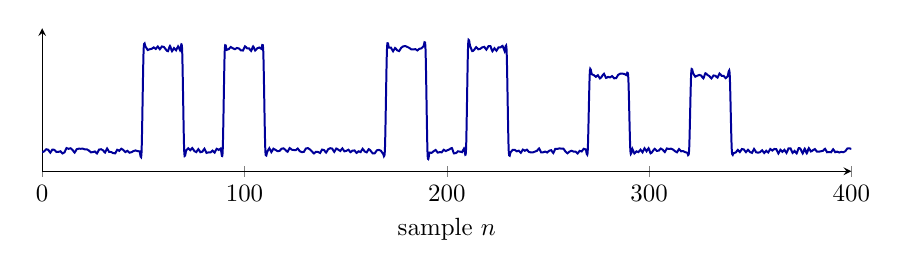
\begin{tikzpicture}[scale=0.9]
  \begin{axis}[width=13cm, height=3.6cm, ymin=0, ymax=1.05,
    xlabel={sample $n$}, ylabel={},
    ytick={\empty}, xtick={0, 100, 200, 300, 400},
    axis y line=left, axis x line=bottom, legend style={font=\scriptsize}]
    \addplot[blue!60!black, thick, smooth, samples=400, domain=0:400]
      { 0.15 + 0.02*rand + (x>50 && x<70 ? 0.75 : 0) + (x>90 && x<110 ? 0.75 : 0)
              + (x>170 && x<190 ? 0.75 : 0) + (x>210 && x<230 ? 0.75 : 0)
              + (x>270 && x<290 ? 0.55 : 0) + (x>320 && x<340 ? 0.55 : 0) };
  \end{axis}
\end{tikzpicture}
\end{center}

Preamble pulses form the four tall bars near the left; the payload that
follows is lower amplitude here to keep the sketch readable.

\subsection{Matched preamble correlator}\label{sec:corr}

The correlator scores every candidate offset $k$ by summing the
envelope inside the four expected pulse windows and subtracting the
energy in the four expected \emph{dead} windows:
\begin{equation}
C[k] = \underbrace{\sum_{t\in \mathcal{P}}\!e[k+t]}_{\text{4 pulses}}
     \;-\;
       \underbrace{\sum_{t\in \mathcal{D}}\!e[k+t]}_{\text{dead slots}} .
\end{equation}
where $\mathcal{P}$ and $\mathcal{D}$ are the sample offsets that
correspond to the pulse-on and pulse-off regions of the preamble
template. A frame candidate at $k$ passes when
$C[k] > \tau$ \emph{and} $C[k]$ is a local maximum
(taller than $C[k\pm 1]$).

\begin{center}
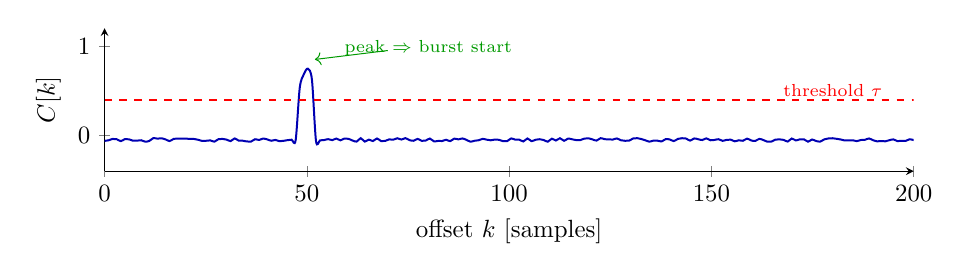
\begin{tikzpicture}[scale=0.9]
  \begin{axis}[width=13cm, height=3.6cm, ymin=-0.4, ymax=1.2,
    xlabel={offset $k$ [samples]}, ylabel={$C[k]$},
    xtick={0, 50, 100, 150, 200}, ytick={0,1},
    axis y line=left, axis x line=bottom]
    % Correlator output — flat noise with peak at ~50
    \addplot[blue!70!black, thick, smooth, samples=200, domain=0:200]
      { 0.02*rand - 0.05 + (x>48 && x<52 ? 0.85 - 0.15*abs(x-50) : 0) };
    \draw[red, dashed, thick] (axis cs:0,0.4) -- (axis cs:200,0.4);
    \node[red, font=\scriptsize] at (axis cs:180,0.5) {threshold $\tau$};
    \draw[green!60!black, ->] (axis cs:70,0.95) -- (axis cs:52,0.85);
    \node[green!60!black, font=\scriptsize] at (axis cs:80,0.98) {peak $\Rightarrow$ burst start};
  \end{axis}
\end{tikzpicture}
\end{center}

\subsection{Threshold and false-alarm control}

The threshold $\tau$ is scaled from a running mean of the correlator
output (analogous to an adaptive noise floor).  Too low and thousands
of noise bumps queue up for CRC checks (each one is
$\sim\SI{50}{\micro s}$ of pointless PPM); too high and weak but
otherwise-valid frames get missed.

\begin{center}
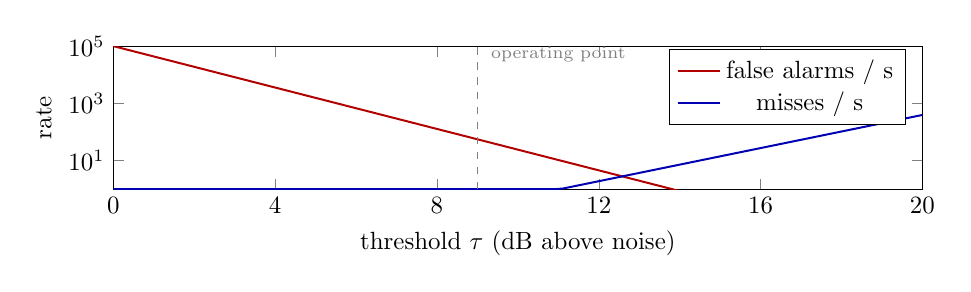
\begin{tikzpicture}[scale=0.9]
  \begin{axis}[width=13cm, height=3.6cm, ymode=log, log basis y=10,
    xlabel={threshold $\tau$ (dB above noise)},
    ylabel={rate},
    ymin=1, ymax=100000, xmin=0, xmax=20,
    xtick={0,4,8,12,16,20}]
    % False-alarm rate falls exponentially
    \addplot[red!70!black, thick, samples=100, domain=0:20]
      { 100000 * exp(-x/1.2) };
    \addlegendentry{false alarms / s}
    % Miss rate rises past ~10 dB
    \addplot[blue!70!black, thick, samples=100, domain=0:20]
      { max(1, 0.5 * exp((x-10)/1.5)) };
    \addlegendentry{misses / s}
    \draw[gray, dashed] (axis cs:9,1) -- (axis cs:9,100000);
    \node[font=\scriptsize, gray] at (axis cs:11,50000) {operating point};
  \end{axis}
\end{tikzpicture}
\end{center}

The operating point in the plot ($\tau \approx \SI{9}{dB}$) is where the
false-alarm curve has fallen enough for the CRC filter (\S\ref{sec:crc})
to absorb the remaining candidates cheaply, while the miss curve is
still flat.

%═══════════════════════════════════════════════════════════════════
\section{PPM bit-slicing}
%═══════════════════════════════════════════════════════════════════

\subsection{Half-slot integration}

Given a burst-start sample index $k_0$ (from the correlator) and a
samples-per-symbol $sps$, iterate through the 112 (or 56) bit slots.
For each slot $i$:

\begin{equation}
P_0^{(i)} \;=\!\!\!\! \sum_{n=k_0 + i\cdot sps}^{k_0 + i\cdot sps + sps/2 - 1}\!\!\!\!\! e[n],
\qquad
P_1^{(i)} \;=\!\!\!\!\!\! \sum_{n=k_0 + i\cdot sps + sps/2}^{k_0 + (i+1)\cdot sps - 1}\!\!\!\!\!\! e[n].
\end{equation}

The slice is a straight comparison, giving one bit per slot:

\begin{center}
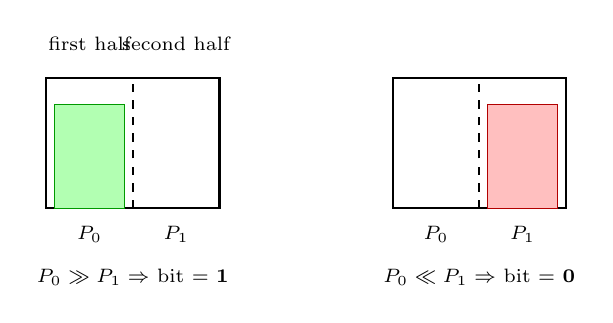
\begin{tikzpicture}[scale=1.1]
  % Draw two adjacent 1 µs cells side by side
  \draw[thick] (0,0) rectangle (2,1.5);
  \draw[thick, dashed] (1,0) -- (1,1.5);
  \node[font=\scriptsize] at (0.5,-0.3) {$P_0$};
  \node[font=\scriptsize] at (1.5,-0.3) {$P_1$};
  \node[font=\scriptsize] at (0.5, 1.9) {first half};
  \node[font=\scriptsize] at (1.5, 1.9) {second half};
  \filldraw[fill=green!30, draw=green!60!black] (0.1,0) rectangle (0.9,1.2);
  \node at (1.0, -0.8) {\scriptsize $P_0 \gg P_1 \Rightarrow$ bit = \textbf{1}};

  % Second cell (bit = 0)
  \begin{scope}[xshift=4cm]
    \draw[thick] (0,0) rectangle (2,1.5);
    \draw[thick, dashed] (1,0) -- (1,1.5);
    \node[font=\scriptsize] at (0.5,-0.3) {$P_0$};
    \node[font=\scriptsize] at (1.5,-0.3) {$P_1$};
    \filldraw[fill=red!25, draw=red!70!black] (1.1,0) rectangle (1.9,1.2);
    \node at (1.0, -0.8) {\scriptsize $P_0 \ll P_1 \Rightarrow$ bit = \textbf{0}};
  \end{scope}
\end{tikzpicture}
\end{center}

\subsection{Soft confidence}

The margin $|P_0 - P_1| \,/\, (P_0 + P_1)$ gives a per-bit confidence
that later stages can use to try error-correction by flipping the least
confident bits (see \S\ref{sec:crc-repair}).  Values near~1 mean a
clean, unambiguous pulse; values near~0 mean the two halves are almost
equal (noise, or two overlapping frames).

\begin{center}
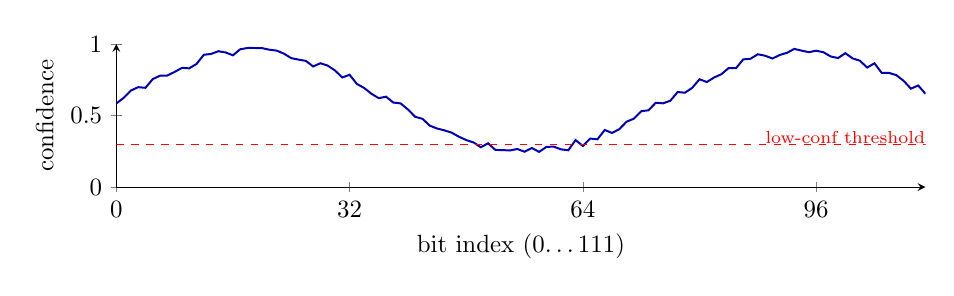
\begin{tikzpicture}[scale=0.9]
  \begin{axis}[width=13cm, height=3.6cm, ymin=0, ymax=1,
    xlabel={bit index (0\ldots 111)}, ylabel={confidence},
    xtick={0,32,64,96,112}, ytick={0,0.5,1},
    axis y line=left, axis x line=bottom]
    \addplot[blue!70!black, thick, samples=112, domain=0:111]
      { 0.6 + 0.35*sin(deg(x/12)) + 0.03*rand };
    \draw[red, dashed] (axis cs:0,0.3) -- (axis cs:111,0.3);
    \node[red, font=\scriptsize] at (axis cs:100,0.35) {low-conf threshold};
  \end{axis}
\end{tikzpicture}
\end{center}

%═══════════════════════════════════════════════════════════════════
\section{CRC-24 and error handling}\label{sec:crc}
%═══════════════════════════════════════════════════════════════════

\subsection{Generator polynomial}

Mode~S uses the fixed generator
\begin{equation}
G(x) = x^{24} + x^{23} + \ldots + x^{3} + 1
     \;\equiv\; \texttt{0x1FFF409}.
\end{equation}
For a 112-bit long frame, the transmitter divides the first
$112-24 = 88$ bits (DF + CA + ICAO + ME) by $G(x)$ modulo~2 and
appends the 24-bit remainder as the PI field.  Receive-side, we do
the same division on the full 112 bits and expect a zero remainder.

\begin{center}
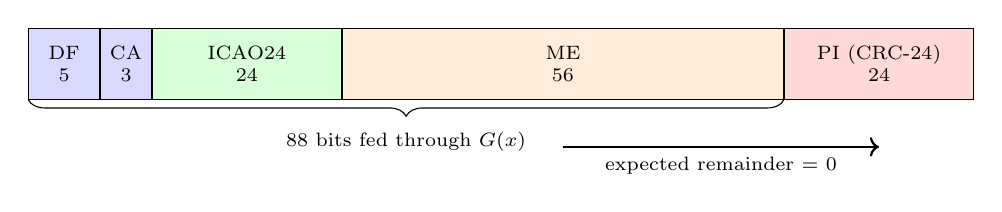
\begin{tikzpicture}[node distance=0mm,
  block/.style={draw, minimum height=0.9cm, align=center, font=\scriptsize}]
  \node[block, fill=blue!15, minimum width=0.9cm]                     (df)  {DF\\5};
  \node[block, fill=blue!15, minimum width=0.6cm, right=0mm of df]    (ca)  {CA\\3};
  \node[block, fill=green!15, minimum width=2.4cm, right=0mm of ca]   (ic)  {ICAO24\\24};
  \node[block, fill=orange!15, minimum width=5.6cm, right=0mm of ic]  (me)  {ME\\56};
  \node[block, fill=red!15, minimum width=2.4cm, right=0mm of me]     (pi)  {PI (CRC-24)\\24};
  \draw[decorate, decoration={brace, amplitude=6pt, mirror}]
     (df.south west) -- (me.south east)
     node[midway, below=8pt, font=\scriptsize]{88 bits fed through $G(x)$};
  \draw[->, thick] ($(me.south)+(0,-0.6)$) -- ($(pi.south)+(0,-0.6)$)
     node[midway, below, font=\scriptsize]{expected remainder = 0};
\end{tikzpicture}
\end{center}

\subsection{Address-XOR trick (DF11)}

For short DF11 replies -- and Mode-S \emph{interrogator} replies -- the
CRC is XOR'd with the target's 24-bit address before transmission.
On receive, dividing by $G(x)$ leaves the address itself in the
remainder.  That means the same routine that validates ADS-B frames
returns an aircraft identity for short-format replies -- useful for
aircraft that transmit brief acknowledgements more often than full
squitters.

\subsection{Error repair by bit flipping}\label{sec:crc-repair}

Since there is no forward error correction, a single bit flip breaks
the frame.  A cheap repair is to identify the $\leq 5$ least-confident
bit positions (from \S{6.2}), flip them one at a time (or in pairs),
and re-check the CRC.  Every additional flip multiplies the syndrome
computation cost -- but Mode~S's CRC is fast (a table of 256 entries),
so up to two-bit repair is affordable at the observed frame rates.

\begin{center}
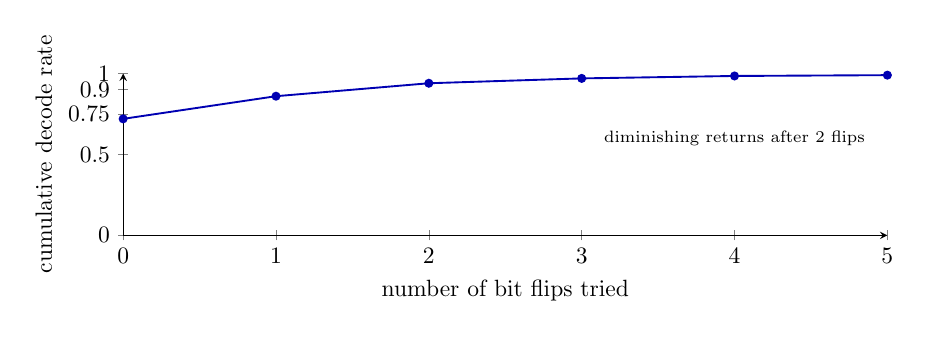
\begin{tikzpicture}[scale=0.85]
  \begin{axis}[width=13cm, height=4cm, ymin=0, ymax=1,
    xlabel={number of bit flips tried}, ylabel={cumulative decode rate},
    xtick={0,1,2,3,4,5}, ytick={0,0.5,0.75,0.9,1.0},
    axis y line=left, axis x line=bottom]
    \addplot[blue!70!black, thick, mark=*, mark size=1.5pt]
      coordinates {(0,0.72)(1,0.86)(2,0.94)(3,0.97)(4,0.985)(5,0.99)};
    \node[font=\scriptsize] at (axis cs:4,0.6)
      {diminishing returns after 2 flips};
  \end{axis}
\end{tikzpicture}
\end{center}

%═══════════════════════════════════════════════════════════════════
\section{DF17 message parsing}
%═══════════════════════════════════════════════════════════════════

\subsection{Type code dispatch}

DF17's 56-bit \texttt{ME} field starts with a 5-bit \emph{type code}
(TC), which chooses the sub-format for the remaining 51 bits:

\begin{center}
\begin{tabular}{r l l}
\toprule
\textbf{TC} & \textbf{Meaning}                & \textbf{Extracted fields}          \\
\midrule
1--4        & Aircraft identification         & callsign (8 chars, ASCII-6)        \\
5--8        & Surface position                 & lat / lon (CPR)                     \\
9--18       & Airborne position (baro alt)    & lat / lon (CPR), altitude          \\
19          & Airborne velocity                & speed, heading, vertical rate      \\
20--22      & Airborne position (GNSS alt)    & lat / lon (CPR), altitude          \\
23--27      & Reserved                         & --                                  \\
28          & Aircraft status                  & emergency, squawk                   \\
29          & Target state and status          & selected altitude, heading         \\
31          & Aircraft operational status      & version, capability                 \\
\bottomrule
\end{tabular}
\end{center}

\begin{center}
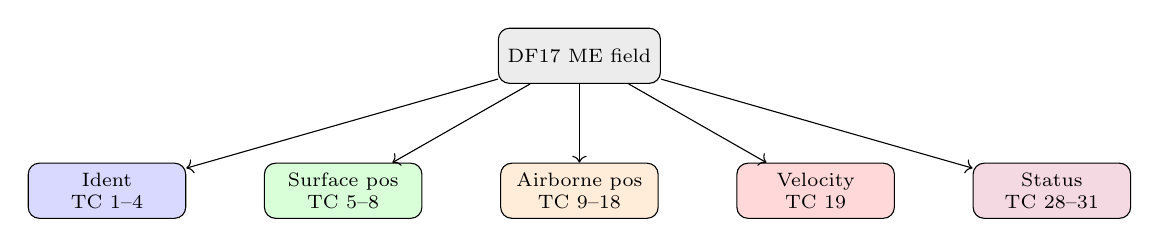
\begin{tikzpicture}[scale=0.95, node distance=0.25cm and 0.4cm,
  leaf/.style={draw, rounded corners, minimum width=2cm, minimum height=0.7cm,
               align=center, font=\scriptsize}]
  \node[leaf, fill=gray!15] (root) {DF17 ME field};
  \node[leaf, fill=blue!15,   below=1cm of root, xshift=-6cm] (id)  {Ident\\TC 1--4};
  \node[leaf, fill=green!15,  below=1cm of root, xshift=-3cm] (sp)  {Surface pos\\TC 5--8};
  \node[leaf, fill=orange!15, below=1cm of root, xshift=0cm ] (ap)  {Airborne pos\\TC 9--18};
  \node[leaf, fill=red!15,    below=1cm of root, xshift=3cm ] (v)   {Velocity\\TC 19};
  \node[leaf, fill=purple!15, below=1cm of root, xshift=6cm ] (st)  {Status\\TC 28--31};
  \foreach \n in {id, sp, ap, v, st}
    \draw[->] (root) -- (\n);
\end{tikzpicture}
\end{center}

\subsection{Callsign (TC 1--4)}

The 48-bit callsign field encodes 8 characters at 6 bits each from a
restricted alphabet (\texttt{A..Z 0..9 <space>}). Decoded straightforwardly with
a lookup table; trailing spaces are trimmed for display.

\begin{center}
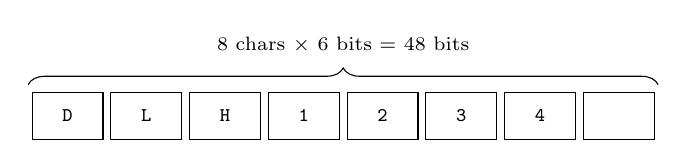
\begin{tikzpicture}[node distance=0mm,
  cell/.style={draw, minimum width=0.9cm, minimum height=0.6cm, font=\scriptsize\ttfamily}]
  \foreach \i/\c in {0/D, 1/L, 2/H, 3/1, 4/2, 5/3, 6/4, 7/\hspace{2pt}}{
    \node[cell] at (\i,0) {\c};
  }
  \draw[decorate, decoration={brace, amplitude=6pt}]
    (-0.5,0.4) -- (7.5,0.4) node[midway, above=8pt, font=\scriptsize]{8 chars $\times$ 6 bits = 48 bits};
\end{tikzpicture}
\end{center}

\subsection{Airborne position and CPR}

Position is transmitted in \emph{Compact Position Reporting} (CPR)
format: 17 bits of latitude + 17 bits of longitude, from which
absolute lat/lon must be reconstructed.  Because 17 bits per axis
covers only about $\pm 3^\circ$ unambiguously, CPR alternates between
two encodings (\emph{even} and \emph{odd}) with slightly different bin
sizes.  Two schemes are used to recover the absolute position:

\begin{itemize}
  \item \textbf{Global} decoding: pairs one even and one odd frame from
        the \emph{same aircraft} within about \SI{10}{s}.  Solves a
        simultaneous equation to yield lat/lon unambiguously worldwide.
        Requires two frames.
  \item \textbf{Local} decoding: uses a recent known reference position
        (either the previous global fix, or the receiver's antenna
        location) to disambiguate a single frame.  Only accurate if
        the aircraft is within $\sim\SI{180}{km}$ of the reference.
\end{itemize}

\begin{center}
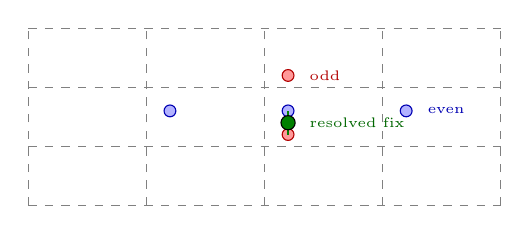
\begin{tikzpicture}[scale=1.5]
  % A grid of NL zones (latitude bands)
  \foreach \y in {0,0.5,1.0,1.5}
    \draw[gray, dashed] (0,\y) -- (4,\y);
  \foreach \x in {0,1,2,3,4}
    \draw[gray, dashed] (\x,0) -- (\x,1.5);
  % Even frame lands ambiguously in one of several cells
  \filldraw[fill=blue!30,   draw=blue!70!black]   (1.2,0.8) circle (0.05);
  \filldraw[fill=blue!30,   draw=blue!70!black]   (2.2,0.8) circle (0.05);
  \filldraw[fill=blue!30,   draw=blue!70!black]   (3.2,0.8) circle (0.05);
  \node[blue!70!black, font=\tiny, right] at (3.3,0.8) {even};
  % Odd frame narrows it down
  \filldraw[fill=red!40,    draw=red!70!black]    (2.2,0.6) circle (0.05);
  \filldraw[fill=red!40,    draw=red!70!black]    (2.2,1.1) circle (0.05);
  \node[red!70!black,  font=\tiny, right] at (2.3,1.1) {odd};
  % Intersection = unique
  \draw[green!50!black, thick] (2.2,0.6) -- (2.2,0.8);
  \filldraw[fill=green!50!black] (2.2,0.7) circle (0.06);
  \node[green!40!black, font=\tiny, right] at (2.3,0.7) {resolved fix};
\end{tikzpicture}
\end{center}

\subsection{Altitude decoding}

The 12-bit altitude field (\texttt{AC}) encodes barometric altitude in
25-foot or 100-foot increments depending on a Q-bit:
\begin{equation}
\text{alt}_{ft} =
  \begin{cases}
    25 \cdot N - 1000       & Q = 1\;(\text{fine, up to } 50\,175\,\text{ft})\\
    100 \cdot \text{Gillham}(N) - 1000
                            & Q = 0\;(\text{coarse, Gillham code})
  \end{cases}
\end{equation}
Almost every modern civilian aircraft uses $Q=1$; Gillham decoding is
only needed for very old transponders.

\subsection{Velocity (TC 19)}

TC-19 messages carry either \emph{ground-referenced} (subtype 1--2:
east/west velocity, north/south velocity) or \emph{airspeed-referenced}
(subtype 3--4: heading + IAS/TAS) plus a vertical rate.  The plugin
computes ground speed and true-track from
\begin{equation}
v = \sqrt{v_{EW}^{2} + v_{NS}^{2}},
\qquad
\theta = \arctan\!\left(\frac{v_{EW}}{v_{NS}}\right).
\end{equation}

\begin{center}
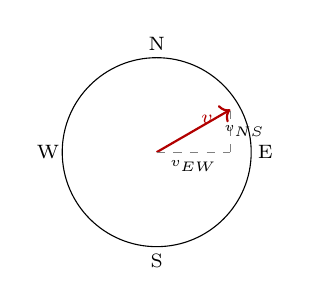
\begin{tikzpicture}[scale=1.2]
  % Compass with velocity vector
  \draw (0,0) circle (1);
  \foreach \deg/\lbl in {90/N, 0/E, 270/S, 180/W}{
    \node at ({1.15*cos(\deg)}, {1.15*sin(\deg)}) {\scriptsize \lbl};
  }
  % Vector at 60° from north (i.e. 30° above E)
  \draw[->, red!70!black, thick] (0,0) -- ({0.9*cos(30)},{0.9*sin(30)});
  \draw[dashed, gray] (0,0) -- ({0.9*cos(30)},0);
  \draw[dashed, gray] ({0.9*cos(30)},0) -- ({0.9*cos(30)},{0.9*sin(30)});
  \node[red!70!black, font=\scriptsize] at ({0.5*cos(30)+0.1},{0.5*sin(30)+0.1}) {$v$};
  \node[font=\tiny] at ({0.9*cos(30)/2}, -0.15) {$v_{EW}$};
  \node[font=\tiny] at ({0.9*cos(30)+0.15}, {0.9*sin(30)/2}) {$v_{NS}$};
\end{tikzpicture}
\end{center}

%═══════════════════════════════════════════════════════════════════
\section{Aircraft tracking and de-duplication}
%═══════════════════════════════════════════════════════════════════

Successive frames from the same ICAO24 update an in-memory record.
Records are \emph{never} time-expired --- once an aircraft is heard it
stays in the table for the whole session (the display sorts by
last-seen so recently-active planes stay on top and long-silent ones
sink to the bottom).  Press \texttt{r} to clear the table on demand.

Each merge is also mirrored to \texttt{plugins/adsb/adsb\_logs/adsb.csv}
as a new row whenever any tracked field (\texttt{lat}, \texttt{lon},
\texttt{alt}, \texttt{gs}/\texttt{ias}/\texttt{tas}, \texttt{heading},
\texttt{vr}, or \texttt{callsign}) actually changed --- see
\S\ref{sec:log} for the schema.

\begin{center}
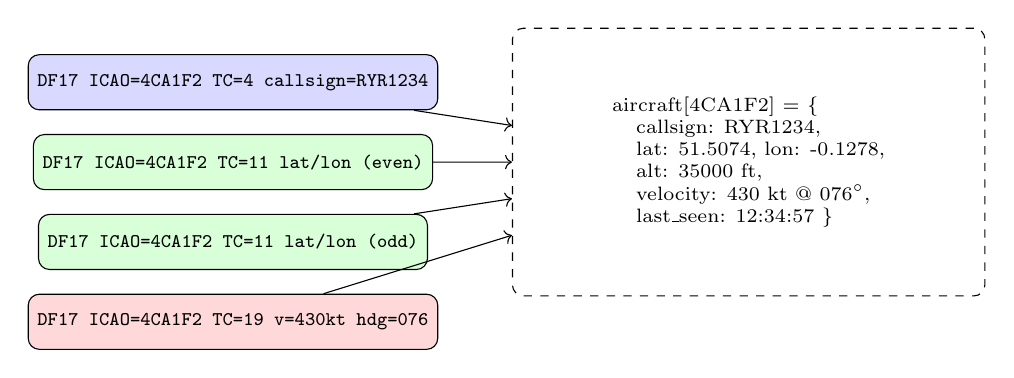
\begin{tikzpicture}[node distance=0.3cm, scale=0.9,
  frame/.style={draw, rounded corners, minimum height=0.7cm, font=\scriptsize\ttfamily}]
  \node[frame, fill=blue!15] (m1) {DF17 ICAO=4CA1F2 TC=4 callsign=RYR1234};
  \node[frame, fill=green!15, below=of m1] (m2) {DF17 ICAO=4CA1F2 TC=11 lat/lon (even)};
  \node[frame, fill=green!15, below=of m2] (m3) {DF17 ICAO=4CA1F2 TC=11 lat/lon (odd)};
  \node[frame, fill=red!15,   below=of m3] (m4) {DF17 ICAO=4CA1F2 TC=19 v=430kt hdg=076};

  \node[right=1cm of m2, minimum width=6cm, minimum height=3.4cm,
        draw, dashed, rounded corners, align=left, font=\scriptsize] (rec)
    {aircraft[4CA1F2] = \{ \\
     \hspace{6pt} callsign: RYR1234, \\
     \hspace{6pt} lat: 51.5074, lon: -0.1278, \\
     \hspace{6pt} alt: 35000 ft, \\
     \hspace{6pt} velocity: 430 kt @ 076$^\circ$, \\
     \hspace{6pt} last\_seen: 12:34:57 \}};
  \draw[->] (m1) -- (rec);
  \draw[->] (m2) -- (rec);
  \draw[->] (m3) -- (rec);
  \draw[->] (m4) -- (rec);
\end{tikzpicture}
\end{center}

%═══════════════════════════════════════════════════════════════════
\section{Persistent CSV log}\label{sec:log}
%═══════════════════════════════════════════════════════════════════

Every meaningful merge of the in-memory record is appended to a
single, always-growing file:

\begin{center}
\texttt{plugins/adsb/adsb\_logs/adsb.csv}
\end{center}

The file is opened with append mode and never rotated, so successive
SDRTerm sessions keep extending the same history.  The \texttt{s} key
in the ADS-B tab toggles logging on and off at runtime, and the toggle
is persisted into the SDRTerm preset via \texttt{save\_state()}.

\subsection{Schema}

Column order (comma-separated, one line per change):

\begin{center}
\begin{tabular}{l l}
\toprule
Column & Content \\
\midrule
\texttt{timestamp} & ISO 8601 UTC, millisecond precision (e.g.\ \texttt{2026-08-08T14:23:12.559Z}) \\
\texttt{icao}      & 6-hex ICAO24 identifier                                                    \\
\texttt{callsign}  & aircraft callsign, blank until an identification frame arrives             \\
\texttt{lat}       & decimal degrees, blank until first CPR global decode                       \\
\texttt{lon}       & decimal degrees                                                            \\
\texttt{alt}       & barometric altitude in feet                                                \\
\texttt{gs}        & ground speed (kt) --- filled from TC=19 subtype 1 / 2                      \\
\texttt{ias}       & indicated airspeed (kt) --- from TC=19 subtype 3 / 4, bit 24 = 0           \\
\texttt{tas}       & true airspeed (kt) --- from TC=19 subtype 3 / 4, bit 24 = 1                \\
\texttt{heading}   & degrees clockwise from north (ground track or magnetic, per subtype)       \\
\texttt{vr}        & vertical rate in feet per minute (signed)                                  \\
\bottomrule
\end{tabular}
\end{center}

\subsection{Row-write rule}

A new row is appended iff either

\begin{itemize}
\item it is the first squitter ever seen from this \texttt{icao} (the
      timestamp is proof-of-hearing even if the frame carries no
      telemetry), or
\item the merged snapshot (all nine tracked fields plus
      \texttt{callsign}) differs from the last-written row for the
      same \texttt{icao}.
\end{itemize}

Three separate speed columns are what keeps the log clean when a
transmitter switches between ground- and airspeed-referenced velocity
messages.  With a single \texttt{speed} column, a switch from
$\text{GS}=380$ to $\text{IAS}=380$ would appear as ``no change''
(losing the type information) while a switch from $\text{GS}=380$ to
$\text{IAS}=390$ would spuriously invalidate the previous ground-speed
reading.  Split slots preserve both: the \texttt{gs} column holds the
last GS reading indefinitely until a fresh GS frame arrives, and the
same for \texttt{ias} and \texttt{tas}.

\subsection{Filtering and plotting}

The ISO-8601 timestamp is lexicographically sortable, so simple
time-range queries need no parsing:

\begin{lstlisting}[language=Python]
import pandas as pd
df = pd.read_csv('plugins/adsb/adsb_logs/adsb.csv',
                 parse_dates=['timestamp'])
window = df[(df.timestamp >= '2026-08-08T14:00:00Z') &
            (df.timestamp <= '2026-08-08T15:30:00Z')]
for icao, path in window.dropna(subset=['lat','lon']).groupby('icao'):
    plt.plot(path.lon, path.lat, label=path.callsign.dropna().iloc[-1])
\end{lstlisting}

%═══════════════════════════════════════════════════════════════════
\section{Worked example}
%═══════════════════════════════════════════════════════════════════

Take the \SI{112}{bit} frame (hex form, MSB first)
\begin{center}
  \texttt{8D4840D6202CC371C32CE0576098}
\end{center}
Its 14 bytes decode as:

\begin{center}
\begin{tabular}{l l}
\toprule
Byte  & Meaning                                             \\
\midrule
\texttt{8D}                       & DF=17, CA=5 (level 2 transponder)             \\
\texttt{48\,40\,D6}                 & ICAO24 = \texttt{4840D6}                       \\
\texttt{20\,2C\,C3\,71\,C3\,2C\,E0}   & ME field: TC=4 (identification), callsign      \\
                                  & = \texttt{"KLM1023 "}                          \\
\texttt{57\,60\,98}                 & PI (CRC-24)                                    \\
\bottomrule
\end{tabular}
\end{center}

Computing the CRC of the first 88 bits gives \texttt{576098}, matching
the transmitted PI -- frame accepted.  The aircraft table gains an
entry
\begin{center}
\texttt{4840D6  KLM1023}
\end{center}
that later positional and velocity frames from the same ICAO will
fill in.

%═══════════════════════════════════════════════════════════════════
\section{End-to-end block diagram}
%═══════════════════════════════════════════════════════════════════

\begin{center}
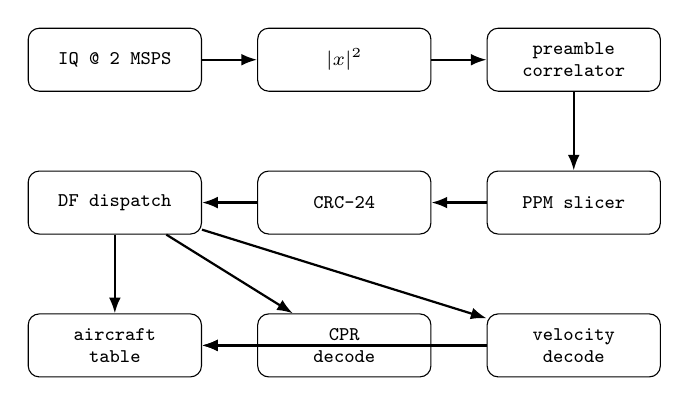
\begin{tikzpicture}[node distance=0.4cm and 0.7cm,
  block/.style={draw, rounded corners, minimum width=2.2cm, minimum height=0.8cm,
                align=center, font=\scriptsize\ttfamily},
  data/.style={font=\scriptsize},
  arrow/.style={-{Latex[length=2mm]}, thick}]

  \node[block] (rf)   {IQ @ 2 MSPS};
  \node[block, right=of rf]  (env)  {$|x|^{2}$};
  \node[block, right=of env] (cor)  {preamble\\correlator};
  \node[block, below=1cm of cor]    (slice){PPM slicer};
  \node[block, left=of slice]       (crc)  {CRC-24};
  \node[block, left=of crc]         (dfd)  {DF dispatch};
  \node[block, below=1cm of dfd]    (tab)  {aircraft\\table};
  \node[block, right=of tab]        (pos)  {CPR\\decode};
  \node[block, right=of pos]        (vel)  {velocity\\decode};

  \draw[arrow] (rf)  -- (env);
  \draw[arrow] (env) -- (cor);
  \draw[arrow] (cor) -- (slice);
  \draw[arrow] (slice) -- (crc);
  \draw[arrow] (crc) -- (dfd);
  \draw[arrow] (dfd) -- (tab);
  \draw[arrow] (dfd) -- (pos);
  \draw[arrow] (dfd) -- (vel);
  \draw[arrow] (pos) -- (tab);
  \draw[arrow] (vel) -- (tab);
\end{tikzpicture}
\end{center}

%═══════════════════════════════════════════════════════════════════
\section{Performance considerations}
%═══════════════════════════════════════════════════════════════════

Per-second cost distribution at \SI{2}{MSPS} on one core:

\begin{center}
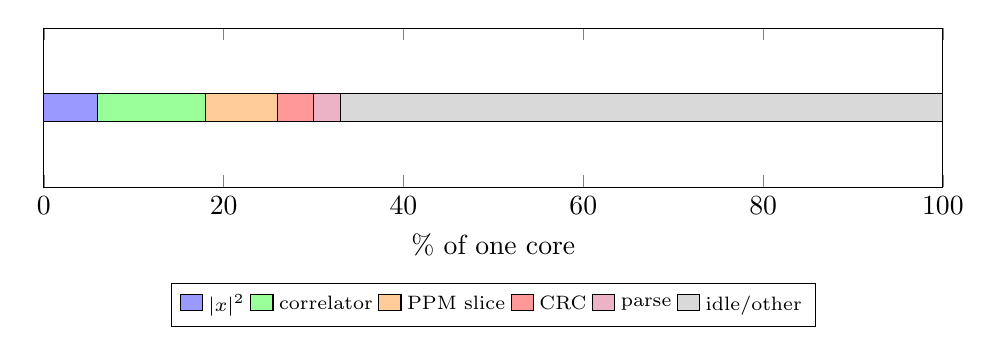
\begin{tikzpicture}
  \begin{axis}[width=13cm, height=3.6cm, xbar stacked,
    ymin=-0.5, ymax=0.5,
    xmin=0, xmax=100,
    ytick=\empty, xtick={0,20,40,60,80,100},
    xlabel={\% of one core},
    legend style={font=\scriptsize, at={(0.5,-0.6)}, anchor=north, legend columns=6}]
    \addplot [fill=blue!40]    coordinates {(6, 0)};    \addlegendentry{$|x|^{2}$}
    \addplot [fill=green!40]   coordinates {(12,0)};   \addlegendentry{correlator}
    \addplot [fill=orange!40]  coordinates {(8, 0)};    \addlegendentry{PPM slice}
    \addplot [fill=red!40]     coordinates {(4, 0)};    \addlegendentry{CRC}
    \addplot [fill=purple!30]  coordinates {(3, 0)};    \addlegendentry{parse}
    \addplot [fill=gray!30]    coordinates {(67,0)};   \addlegendentry{idle/other}
  \end{axis}
\end{tikzpicture}
\end{center}

The correlator dominates -- it runs on every input sample.  With a
dense airport nearby (thousands of candidates/s past $\tau$) the CRC
share rises but stays modest thanks to the byte-wise LUT.

%═══════════════════════════════════════════════════════════════════
\section{References}
%═══════════════════════════════════════════════════════════════════

\begin{enumerate}
  \item ICAO Annex 10, Volume IV, ``Aeronautical Telecommunications --
        Surveillance and Collision Avoidance Systems''.  The
        authoritative Mode-S / ADS-B spec.
  \item RTCA DO-260B, ``Minimum Operational Performance Standards for
        1090 MHz Extended Squitter ADS-B''.
  \item \href{https://mode-s.org/decode/}{\texttt{mode-s.org/decode}}
        -- Junzi Sun's excellent ADS-B decode tutorial and Python
        library, from which several message-format tables in this doc
        are cross-checked.
  \item \texttt{dump1090} -- reference SDR decoder.  The correlator
        design here mirrors its \texttt{demodulate2400.c} logic but
        drops the DSP-specific tricks not portable to Python.
\end{enumerate}

\end{document}
